\subsection{Alloy code}
G1 — Users can register and have a profile in BBP

This goal ensures that the system correctly manages user identities and registration.
The assertion \textit{differentUsersCannotBeSameUser} checks the uniqueness of users, stating that two distinct user instances cannot represent the same logical user. This prevents identity collisions within the system.

The assertion \textit{userRegisteredNotAnonymous} verifies that every registered user is not anonymous. In other words, once a user is registered, both must be associated with a concrete and identifiable profile. Moreover, these assertions guarantee that users in BBP are uniquely identifiable, non-anonymous once registered, and consistently represented throughout model phases.

G2 — Manual path creation

This goal concerns the manual creation of paths by users. The predicate \textit{showPath} models the evolution of the system state. So, initially, no trips are present. Eventually, two trips exist, representing the successful creation and storage of paths. This temporal behavior validates that manual path creation leads to persistent system state changes, confirming the goal. Trips are chosen on the select phase. 

G3 — Automatic path creation

This goal ensures that automatic and manual path creation are mutually exclusive.
The assertion \textit{AutomatedXorManual} expresses an 'exclusive-or' between the two modes. Specifically, if a data w is equal to Automated and at the same time equal to \textit{p.Recorded}, then it must not be equal to Manual. Furthermore, if w is equal to Manual and equal to \textit{p.Recorded}, then it must not be equal to Automated. This allows that a recorded path cannot either automatically and manually created at the same moment. The Alloy analyzer confirms this behavior by finding no counterexamples, meaning the constraint is consistent.

G4 — Browsing and viewing paths

The function \textit{searchPath} retrieves all paths composing a given trip, that it is constrained strictly to 1 by the facts. The predicate \textit{selectPath} calls the function and it ensures that at least one path is available for selection. This confirms that the system can search, retrieve, and select paths corresponding to user-defined criteria, fulfilling the browsing requirement. 

G5 — Recording and storing trips

The function \textit{extractTrip} ensures that each user is associated with at most one trip at a time. The predicate \textit{viewTrip} models the transition from no trips to one trip. These constraints validate that trips are correctly going through the phases, uniquely associated with users, and persist in the system.

G6 — Trip statistics and weather conditions

The predicate \textit{viewTripAtCheckInfo} ensures that a trip eventually exists. Then the trip reaches the \textit{CheckInfo} situation. The trip belongs to the requesting user. This verifies that statistical and contextual information is available and accessible for recorded trips.

G7 — Merging information and generating the optimal path

This goal describes the final phases of application usage, including information merging and path publication. The predicate \textit{show[]} models the evolution of the system over time. Initially, the number of Trip instances is 0, representing the state before any trip is created. At some intermediate point, the number of Trip instances becomes 3, representing multiple partial or candidate trips during processing. Finally, there exists a Trip whose situation is \textit{Publish}, representing the successful generation and publication of the optimal path. Overall, this goal captures the intended steps of the application, from initial usage, through intermediate processing steps, to the final publication of a single optimal trip of a given user.

\begin{lstlisting}[
    style=alloy,
]

abstract sig Status {}
one sig Optimal, Acceptable, Sufficient, Difficult extends Status {}
abstract sig Way{}
one sig Automated, Manual extends Way{}
sig idUser {}
sig idPath{}
sig idTrip{}

enum currentSituation {
		Search, 
		Select, 
		Ride, 
		CheckInfo, 
		Publish
}

var sig Trip {
	var id: one idTrip,
	var ComposedOf: one Path, 
	var BelongingTo: one System,
	var userRelated: one user,
	var situation: one currentSituation
} {
	#ComposedOf = 1
}

sig user {
	id: one idUser,
	var tripInfo: lone Trip
} {
}

sig userAnonymous extends user {
}

sig Path {
	id: idPath,
	var PartOf: set Trip,
	Recorded: one Way,
 	computedStatus: one Status      
} {
}

one sig System {
	ProvidingPaths: set Path,
	toUser: some user
}{	
}

------------------------------ facts on step progression ------------------------------


// Every situation is a ordered step
fun nextSituation[t: Trip]: one currentSituation {
	(t.situation = Search) => Select else
	(t.situation = Select) => Ride else
	(t.situation = Ride) => CheckInfo else
	(t.situation = CheckInfo) => Publish else
	(t.situation = Publish) => Search else none
}

// Recall nextSituation function in order to move along steps
fact stateProgression {
	always (
		all t: Trip |
				t.situation' = t.situation or
 				t.situation' = nextSituation[t] or
 				t not in Trip'
 	)
}

// Every steps appears at select
fact insertingTrip {
	always (
		all t: Trip | 
			once (t.situation = Select) 
	)
}

// Trip rules along steps
fact finalizingTrip {
	always (all t: Trip |  after t.situation = CheckInfo implies eventually (t not in Trip))
	always (all t: Trip | t not in Trip' implies after always t not in Trip')
}

// Trip can't disappear if appears at least once after select
fact persistencyAlongSteps {
  all t: Trip| all cS: t.situation | 
    (cS = Search or cS = Select or cS = Ride or cS = CheckInfo ) implies
      always (t in Trip')
}

fact persistencyPathAlongSteps {
	all t: Trip, s: System | s in t.BelongingTo implies always (s in t'.BelongingTo)
	all t: Trip, u: user | u in t.userRelated implies always (u in t'.userRelated)
	all t: Trip, p: Path | p in t.ComposedOf implies always (p in t'.ComposedOf)
	all t: Trip, idt: idTrip | idt in t.id implies always (idt in t'.id)
}

fact userPersistency {
	user = user' 
}

fact userOfTripRemainsSame {
    always all t: Trip | t'.userRelated = t.userRelated
}

// all user have a unique email address and a unique username
fact uniqueID{
	always ( all disj u1 , u2 : user | u1.id != u2.id )
}

// every Email is associated to one User
fact uniqueID {
	always ( all i : idUser | one u : user | u.id = i )
}
------------------------------------------------------------------------------------------------------

// Relationship between Trip, path and userAnonymous
fact {
	no u: userAnonymous | all t: Trip | all p: Path | p in t.ComposedOf and t in u.tripInfo
}

fact {
	all u: user | all s: System | u in s.toUser
}

fact {
	all t: Trip | all u: user | u in t.userRelated implies (t in u.tripInfo)
}

fact {
	all i: idUser | all u: user | all u2: user | i in u.id and u != u2 implies always(i not in u2.id)
}

// users must appear and be related to trip
fact  {
	all t: Trip | all u: user | u = t.userRelated implies (no t2: Trip | t2 != t and u in t2.userRelated)
	all t: Trip | all u: user | u = t.userRelated implies (no t2: Trip' | t2 != t and u in t2.userRelated)
	all t: Trip | all u: user | u = t.userRelated implies after always (no t2: Trip | t2 != t and u in t2.userRelated)
	all u: user | all t: Trip | u = t.userRelated implies always (t in u.tripInfo)
}

fact  {
	always( all u1: user | all t: Trip | all s: System | t in u1.tripInfo implies (u1 in t.userRelated and u1 in s.toUser and t.ComposedOf in s.ProvidingPaths))
}

fact {
	always(all disj t1, t2: Trip | t1.id != t2.id )
}

fact {
    all t: Path | t.id' = t.id
}

fact userTripHasPath {
	always (all t: Trip | all u: user | t in u.tripInfo implies (all p: Path | p in t.ComposedOf))
}

fact {
	always(all an: userAnonymous | all u: user | an != u)
}

fact {
	all u1, u2: user | all t: Trip | t in u1.tripInfo and u1.id != u2.id implies (t not in u2.tripInfo)
}

// user is quantifiable and unique
fact distintUser {
	all u1, u2: user | u1.id != u2.id iff (u1 != u2)	
	all u1, u2: user | u1 != u2 implies after always u1 != u2		
}

fact {
	all t1, t2: Trip | t1 != t2 implies  t1.id != t2.id
	all t1, t2: Trip | t1 != t2 implies after always t1.id != t2.id
}

// future steps must have same patters of previous steps
fact {
	(all sys: System | all t: Trip | all u: user | sys in t.BelongingTo and u in t.userRelated and t in u.tripInfo and u in sys.toUser implies after always ( System' = t.BelongingTo and user' = t.userRelated and user' = sys.toUser and Trip' = u.tripInfo))
}

-----------------------------------------------------------------------------------------------------

// G1: Users can register and have a profile in BBP application.

assert differentUsersCannotBeSameUser {
 	all u1, u2: user | u1.id  != u2.id implies u1 = u2
}

assert userRegisteredNotAnonymous {
	all u: user | all an: userAnonymous | u = user implies u != an
}

// G2: Users manually create bike paths in an inventory by specifying the name of the streets and the status.

pred showPath {
#Trip = 0
eventually (#Trip = 2) 
}

// G3: Users create bike paths in an automated mode where the system acquire data from the user's mobile device and reconstruct the path.

assert AutomatedXorManual {
	all w: Way | all p: Path | w = Automated and w =  p.Recorded implies (w != Manual)
	all w: Way | all p: Path | w = Manual and w = p.Recorded implies (w != Automated)
}

// G4: Users browse bike paths within the inventory. They can specify an origin and destination and ask the system to visualize the bike path on a map.

fun searchPath[t: Trip]: set Path{
	{
		p: Path | some g: t.ComposedOf | p = g
	}
}

pred selectPath[t: Trip]{
	some searchPath[t] 
}

// G5: Users record their trips and store them to keep track of their cycling activities.

fun extractTrip[u: user]: lone Trip {
    u.tripInfo
}

pred viewTrip [u: user] {
	#Trip = 0
	eventually (#Trip = 1) 
	#extractTrip[u] <= 1
}

// G6: Users can see for a recorded trip various statistical data of the user performances as well as meteorological information during the respective trip.

pred viewTripAtCheckInfo[u: user] {
    #Trip = 0
	eventually ( some t:Trip | #Trip = 1 and t.situation = CheckInfo and  t in u.tripInfo ) 
}

// G7: The system uses information published by the users about the paths by merging pieces of information to generate the optimal path, using the freshness and number of confirmed data.

pred show[] {
    #Trip = 0
    eventually (#Trip = 3) 
    eventually (some t: Trip | t.situation = Publish)
}

//check differentUsersCannotBeSameUser for 2 but exactly 3 user
//check userRegisteredNotAnonymous  for 3 but exactly 3 user
//check AutomatedXorManual for 2
//run viewTripAtCheckInfo for 3 but exactly 3 user
//run showPath for 3 but exactly 3 user
//run viewTrip for 3 but exactly 3 user
//run selectPath for 3 but 1 Path, 5 steps
//run show for 3 but exactly 3 user

\end{lstlisting}

\newpage
\begin{figure}
    \centering
    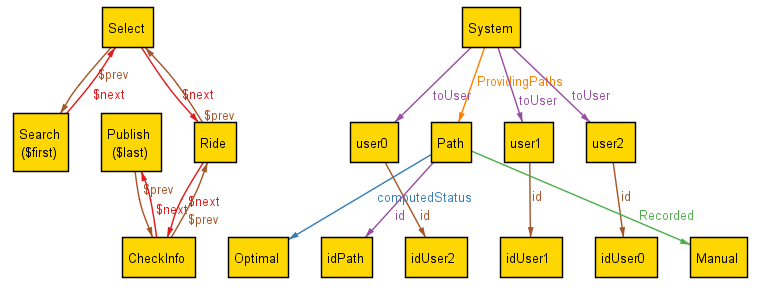
\includegraphics[width=0.5\linewidth]{RASD/Images/imagesAlloy/idleSearchPhase.png}
    \caption{Idle phase}
    \label{fig:placeholder}
\end{figure}

\begin{figure}
    \centering
    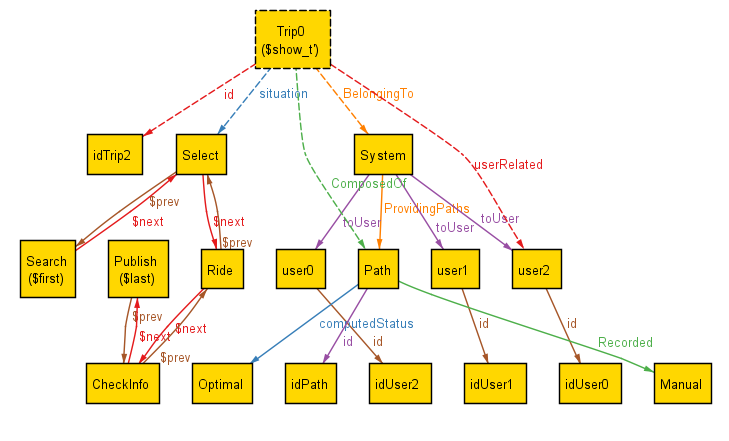
\includegraphics[width=0.5\linewidth]{RASD/Images/imagesAlloy/Select.png}
    \caption{Select Phase}
    \label{fig:placeholder}
\end{figure}

\begin{figure}
    \centering
    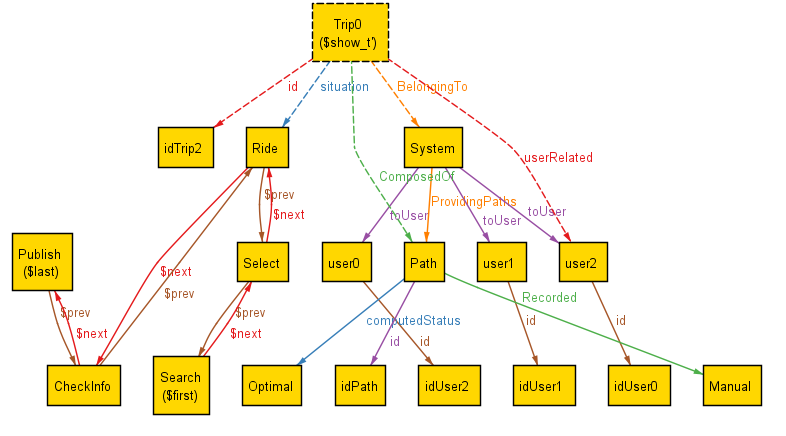
\includegraphics[width=0.5\linewidth]{RASD/Images/imagesAlloy/Ride.png}
    \caption{Ride phase}
    \label{fig:placeholder}
\end{figure}

\begin{figure}
    \centering
    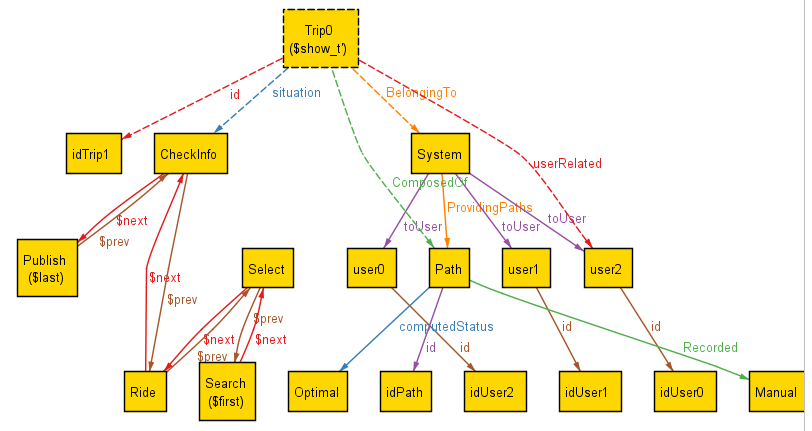
\includegraphics[width=0.5\linewidth]{RASD/Images/imagesAlloy/CheckInfo.png}
    \caption{Checkinfo phase}
    \label{fig:placeholder}
\end{figure}

\begin{figure}
    \centering
    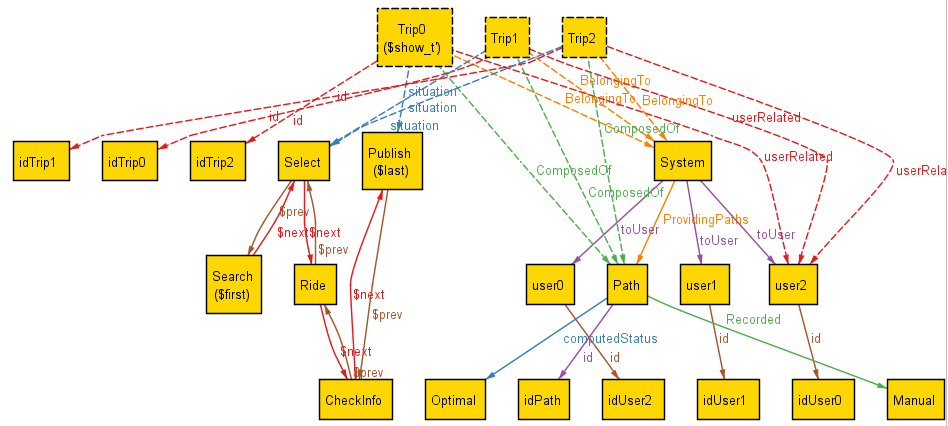
\includegraphics[width=0.5\linewidth]{RASD/Images/imagesAlloy/PublishPhase.png}
    \caption{Publish phase}
    \label{fig:placeholder}
\end{figure}